

\documentclass{sig-alternate-05-2015}

% Include useful packages
\usepackage{graphicx}
\graphicspath{ {images/} }
\usepackage{float}


\begin{document}

% Copyright
\setcopyright{acmcopyright}


\title{Testing and Tuning SkinnyDip: Noise-Robust Clustering}
\numberofauthors{2} 
\author{
% You can go ahead and credit any number of authors here,
% e.g. one 'row of three' or two rows (consisting of one row of three
% and a second row of one, two or three).
%
% The command \alignauthor (no curly braces needed) should
% precede each author name, affiliation/snail-mail address and
% e-mail address. Additionally, tag each line of
% affiliation/address with \affaddr, and tag the
% e-mail address with \email.
%
% only author :(
\alignauthor
Grant King\\
       \email{kinggra1@msu.edu}
}
% There's nothing stopping you putting the seventh, eighth, etc.
% author on the opening page (as the 'third row') but we ask,
% for aesthetic reasons that you place these 'additional authors'
% in the \additional authors block, viz.
\date{28 April 2017}
% Just remember to make sure that the TOTAL number of authors
% is the number that will appear on the first page PLUS the
% number that will appear in the \additionalauthors section.

\maketitle

\begin{figure*}[t]
\centering
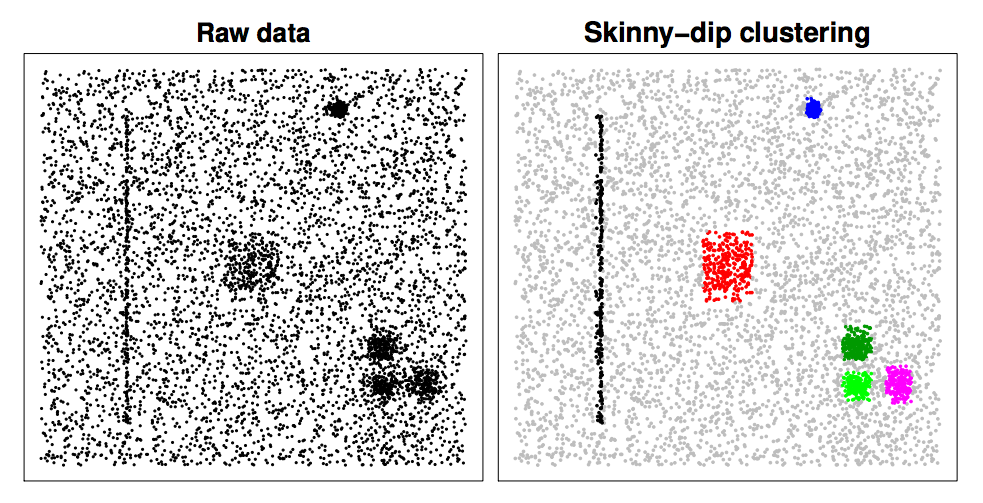
\includegraphics[width=\textwidth]{images/SkinnyDipExample}
\caption{The running example used by Maurus, et al. throughout \cite{skinnydip}}
\label{fig:sdexample}
\end{figure*}

\begin{figure*}[t]
\centering
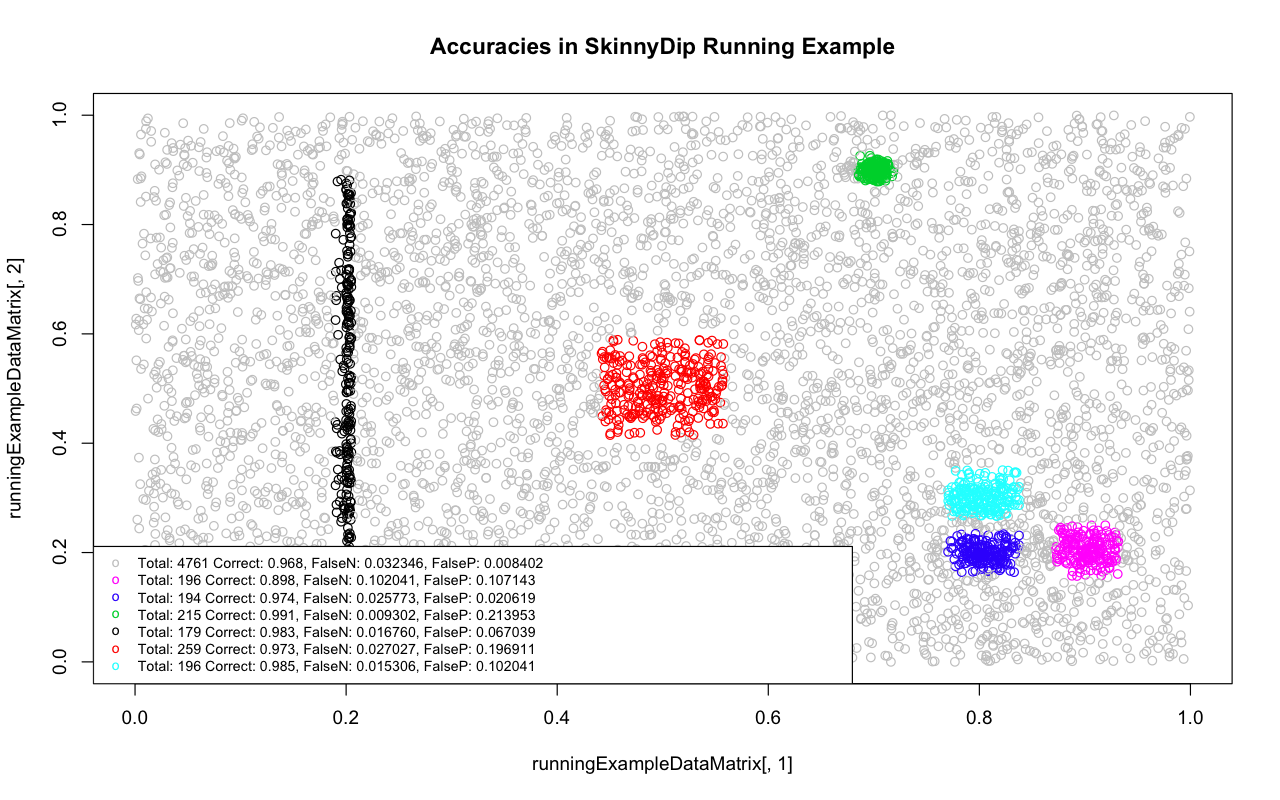
\includegraphics[width=\textwidth]{images/SkinnyDipAccuracy}
\caption{Accuracies of the given SkinnyDip example.}
\label{fig:sdaccuracy}
\end{figure*}

\begin{figure}[t]
\centering
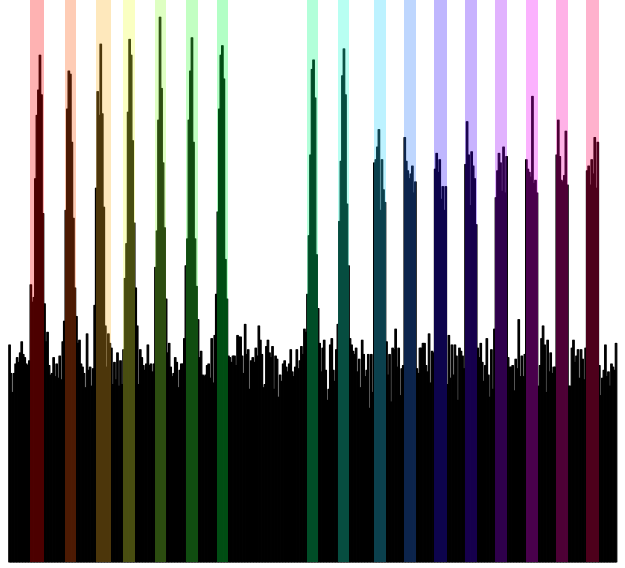
\includegraphics[width=\columnwidth]{images/unimodes}
\caption{Multiple unimodal regions detected with the dip test.}
\label{fig:skinnystripes}
\end{figure}






\section{Problem Description}
It is not uncommon for some real-world data sets to feature an abundance of noise. Depending on the severity of this noise, classical clustering methods may fail due to due to dependence on clean data or confusion from increasingly excessive noise. SkinnyDip is an algorithm proposed by Maurus et al.\cite{skinnydip} designed to handle clustering data in highly noisy environments. SkinnyDip is based on the statistical concept of the \textit{dip} \cite{dip}. 

The dip views the structure of the Empirical Cumulative Distribution Function(ECDF) of a set of single dimensional data to determine whether it is unimodal or multimodal. This test is expanded to a multidimensional, recursive heuristic in order to isolate the various modes of each feature of a set of data. This results in a deterministic, parameter-free, unsupervised method of finding clusters that are based on the modes of multivariate distributions. 

My goal is to study the error present in the existing SkinnyDip algorithm, and then augment it with the addition of a second clustering method in an attempt to improve the error that is present in the hypercubic-bound clusters, and perform additional tests to demonstrate its usefulness on noisy, real-world data sets.


\section{Introduction}
Data clustering is a fundamental problem in Machine Learning, and has been approached in a variety of ways, resulting in a plethora of tools and methods \cite{ClusteringMethods}, many of which are sensitive to noise and other outliers. Additionally, many common techniques, such as k-means clustering, operate as closed set clustering methods and are unable to reject noise at all.

\cite{DBSCAN} is a density-based technique for finding clusters in environments that may contain noise. However, it has the disadvantages of being a parameterized method, and still continues to find extraneous clusters in increasingly noisy data when compared to SkinnyDip.

A single other existing method for clustering using the statistical dip test was found, a technique called DipMeans\cite{dipmeans}. This method takes a different approach to using the dip test by performing it on a collection of distance measurements as opposed to the raw data values themselves. SkinnyDip, however, requires no distance measurements  and is both functionally and computationally distinct from the DipMeans technique.

While SkinnyDip does manage to find all values within a cluster with high accuracy and precision, there is still a notable risk of false classifications for both noise and legitimate classes. This is inherent in the way that the algorithm segments the clusters into hypercubic regions. If the data does not fit a cubic model, then the values included in extreme regions of the cluster (e.g. the corners of a square cluster) are likely to be false positives and should not have been included. Conversely, the hypercubic faces may be likely to segment off data that should be included in the cluster.  This discrepancy increases exponentially as the dimension of the data increases, an issue acknowledged in the original paper\cite{skinnydip}. I plan to demonstrate that the addition of a second reclustering step can reduce the former source of error, with minimal negative impact on the existing true positive matches.

\section{Data} \label{data}
A visual example of the purpose of SkinnyDip is demonstrated in the running example data from \cite{skinnydip} (See Figure \ref{fig:sdexample}) which shows the extraction of distinct shapes from a two-dimensional data field that consists of 80\% static noise. A variety of similar clustering methods were shown to perform poorly on this data set, both through the inclusion of the evenly-distributed, static noise in clusters, and through excessive segmentation of the actual classes.

Aside from the uniform background noise, the running example data consists of 2 distinct cluster models: two rectangular model clusters and four 2D Gaussian model clusters. In Figure \ref{fig:sdexample} the square classes are on the left side of the image and are colored red and black, while the remaining four, smaller clusters are the 2D Gaussians. In the process of generating this data, 200 points are generated using their respective distributions (uniform or normal), and placed on top of the background noise covering the entire field. Any noise that falls within the bounds of these distributions is recategorized as being part of that class.

In the process of testing the existing SkinnyDip results, I created tools to generate Gaussian clusters of arbitrary dimensionality in a field of uniformly random background noise. These were designed to test the inherent error in SkinnyDip's boundaries for normally distributed features, and to further see how this error changed as the dimension of the data increased. For this data, the clusters and background noise were generated, and then any background noise within the ~95\% confidence interval of a cluster (2 standard deviations of the mean) was also classified into that cluster. This leaves us with a zone beyond the ~95\% confidence ellipse that consists of both valid and noise data, which I believe can represent an accurate approximation of realistic clusters.

Any synthetic or real data that will be analyzed using both the original and my augmented version of SkinnyDip should have uniformly random background noise, or there will be clusters falsely detected by variations in the distribution of the background. The algorithm also benefits from a certain degree of density to the background noise, as an increase in even background noise can help flatten out falsely modal areas of noise.

\section{Methodology}
\subsection{SkinnyDip}

The SkinnyDip clustering algorithm is a deterministic, parameter-free, unsupervised method of finding clusters in noisy data. Being based on the $dip$ test, we can look at the ECDF of a single dimension of data at a time. In addition to finding the modality of a region, the dip test also returns the locations of the inflection points that define the unimodal region. The test is a hypothesis test that assumes a particular region is unimodal, and calculates the size of margin of flexibility necessary to create an exclusively unimodal ECDF curve over the data. If this margin is sufficiently large, the hypothesis is rejected in favor of the data being at least bimodal. In order to find each unimodal region in a single dimension, the dip test will recurse into subregions detected to be at least bimodal until termination when the dip test returns a valid unimodal region. Each unimodal result of the dip test represents a different unimodal portion of the data in that dimension, visualized in Figure \ref{fig:skinnystripes}.

Extrapolating this one-dimensional tool to an arbitrary number of dimensions, we can continue to search for modal regions in different dimensions in order to find hyperintervals with which to divide our data. Intuitively, the stripes that are found in each dimension can be overlaid and recombined in order to detect regions of modality in multiple dimensions, indicating the presence and location of a cluster. This algorithm as a worst-case time complexity of $O(n*log(n)*m + n*m*k)$ but the practical run time was demonstrated to grow linearly as $O(n*m)$, as the number of clusters is likely to be much smaller than the number of data points.

The paper goes on to discuss a deterministic method for projecting the data into a space with maximum modality, using a gradient ascent method. This is made deterministic by finding a deterministic initialization for gradient ascent by sampling from a sparse grid. The basis of projection is found one dimension at a time, and once no more valuable dimensions can be found, the projection portion of the algorithm terminates, and the data is then projected into this new space for clustering. SkinnyDip, as described above, is then run in this new space, and the cluster labels are returned. The authors refer to this more complex algorithm as SparseDip.

In my testing, I will only be working with and modifying the result of SkinnyDip, as if I were working in an arbitrary space. Any additional clustering that I do with the results of SkinnyDip can just as easily be performed in the transformed space of SparseDip before the labels are returned, so I will focus my work on minimizing the error of well-formed maximally-modal data.

\subsection{Testing}
My initial hypothesis was that the hypercubic regions returned by the SkinnyDip algorithm would represent an over-classification of noise into the membership of each cluster. As the algorithm returns arbitrary labeled clusters, this first involved finding a way to associate each cluster back to its ground truth membership for comparison. \\

I changed this method to prioritize data point overlap over cluster mean distances. The main motivation of this change was to factor in the actual size of clusters as opposed to just their locations. Additionally, this allows us to confirm whether or not a cluster has successfully been found. Random noise may possibly be falsely classified as a cluster, in which case it will have a meaningful nearest ground truth mean, but the intersection of points in the found and ground truth clusters will not represent the majority of points present in the ground truth cluster. This would indicate that we have found a false cluster relative to the ground truth, but this was not apparent before doing a point-set comparison. In this way, is also possible to set a threshold ratio to determine what is and is not a valid cluster compared to the ground truth. Once the best mapping of detected to ground truth labels had been determined, the SkinnyDip results could be mapped onto the original data and individual label point-sets could be compared. \\

To gather some initial information about the quality of the clusters, I reported a number of statistics about the detected clusters. The reported values included:
\begin{enumerate}
	\item The total number of points placed in the cluster
	\item The percentage of ground truth points detected
	\item The false negative percentage
	\item The false positive percentage
\end{enumerate}
Using these metrics, I expanded upon the authors' reporting by color plotting each of the classified points, and adding a legend with my reported statistics, associated with the respective plot colors. I also wanted to visualize the ground truth values of data I was testing, so I added the option to plot the ground values as well. 


As described in section \ref{data}, the ground truth membership of the synthetic clusters was defined to be the number of points within 2 standard deviations of the cluster mean.
\subsection{Tuning}
As discussed in section \ref{results}, I discovered that the SkinnyDip algorithm was under-classifying valid points into clusters, or equivalently, over-classifying into the noise category from each class. My first idea to correct for this was to incorporate a certain number of nearest adjacent points into a cluster, but I could not think of a good criteria for termination, and realized that this would generally function as inflating the existing cluster in the same hypercubic shape.

My final implementation decision was based on the idea that the contents of these initial cluster regions, although incomplete, would still have information about the underlying structure of the cluster itself. If the cluster has some degree of covariance, then this could still be approximated by using the sample captured in the initial cluster as evidence of the underlying distribution.

For each cluster, I calculated the covariance matrix and then found the Mahalanobis distance of the surrounding points in order to create a new classifications. Mahalnobis distance for point $x$ from cluster mean $\mu$ is defined as:
\begin{center}
$D = \sqrt{(x-\mu)^TS^{-1}(x-\mu)}$ \\
where $S$ is the covariance of the observed cluster points.
\end{center}
Given this definition, I quickly ran into issues with singular covariance matrices, and decided to reformulate to my distance to a Mahalanobis distance measurement to use the Moore-Penrose pseudo-inverse, similar to \cite{Mahalnobis}. Now our Mahalnobis metric is defined as:
\begin{center}
$D = \sqrt{(x-\mu)^TS^+(x-\mu)}$ \\
where $S^+$ is the Moore-Penrose generalized inverse of the empirical covariance matrix, computed via the Single Value Decomposition method.
\end{center}
As the Malahanobis distance for these points represents a generalized measure of standard deviations from the cluster mean, we can set a threshold for membership based on these standard deviations. Typically I would think to find values within 2 or so standard deviations, but our evidence is already and under-approximation of the actual cluster, so we will increase this value to try to approximate the missing data. I initially found that a value of 3 standard deviations worked well as a threshold for the 1D, 2D, and 3D test data that I was visualizing, but when I tried to extrapolate this to higher dimensions, the error quickly returned to the same level present in the original clustering; This was shown in my project presentation on the Conclusion slide. 

Since the presentation, I have adjusted this value to grow exponentially, to accurately track the growth of error in the data. If a certain, consistent portion of data is missed in each dimension, then the under-classification will grow exponentially, which can be visualized by in \ref{fig:falsenegmd}. In order to counteract this, I will exponentially increase the the expansion approximation threshold. After trying a few empirical tests, I settled on the equation: \\
\begin{center}
$t = 1.92+1.08^d$ \\
where $d$ is the dimension of the data
\end{center}
All points with a Mahalanobis distance less than this $t$ are included in the newly approximated cluster.

This augmentation of the SkinnyDip algorithm now adds in the necessity to do distance measurements from each point to each cluster mean, and therefore adds a new dependency of $O(n*k)$ to the runtime. This does not change the worst-case run time of the SkinnyDip algorithm, but it does change the practical runtime, because this $O(n*k)$ calculation is guaranteed and entirely performed for each application of the new algorithm, giving us a new practical runtime of $O(n*(k+m))$, where our practical runtime is now determined by the number of points and both the dimension of the data (for SkinnyDip) and the number of clusters (for reclustering).

Another attempted implementation involved creating a a diagonal covariance matrix based on the variance of each point in a single dimension at a time. This variance matrix would not generalize to arbitrary data well, but I thought it might be a good measurement of how well I could potentially improve the classification error in perfectly independent synthetic data. Interestingly, the classification error for this method was even higher than for the previously described method that accounted for the entire observed covariance, so the idea was readily discarded.







\section{Implementation}
This project was implemented in R, using the existing SkinnyDip library developed by Maurus et. all, which can be found at \cite{skinnycode}. Installation of the library involved sorting out a large set of dependency issues on my computer that ended in a clean install of some command line installers. This was the first time I have ever worked with R, and I decided it would be a worthwhile challenge to learn a new language that I have often heard referenced in the context of data science. A large portion of initial time was spent learning the language while developing the set of functions for remapping and calculating the error on each cluster. Some initial misconceptions about R syntax led to bugs that persisted through the intermediate report. All portions of this project, beyond the SkinnyDip algorithm that returns an initial vector of classification labels, were implemented by myself.


\begin{figure*}[t]
\centering
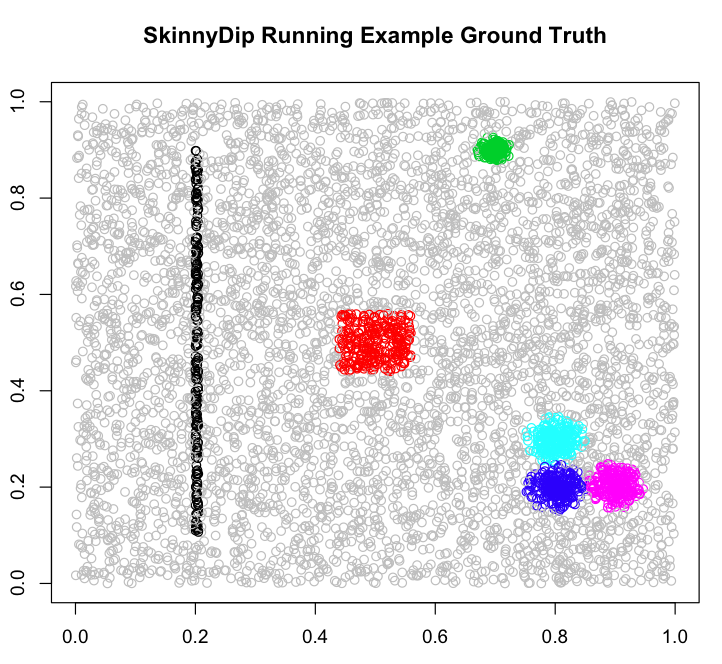
\includegraphics[width=\columnwidth]{images/RunningExampleGT}
\caption{Ground truth values for running example.}
\label{fig:runningGT}
\end{figure*}


\begin{figure*}[t]
\centering
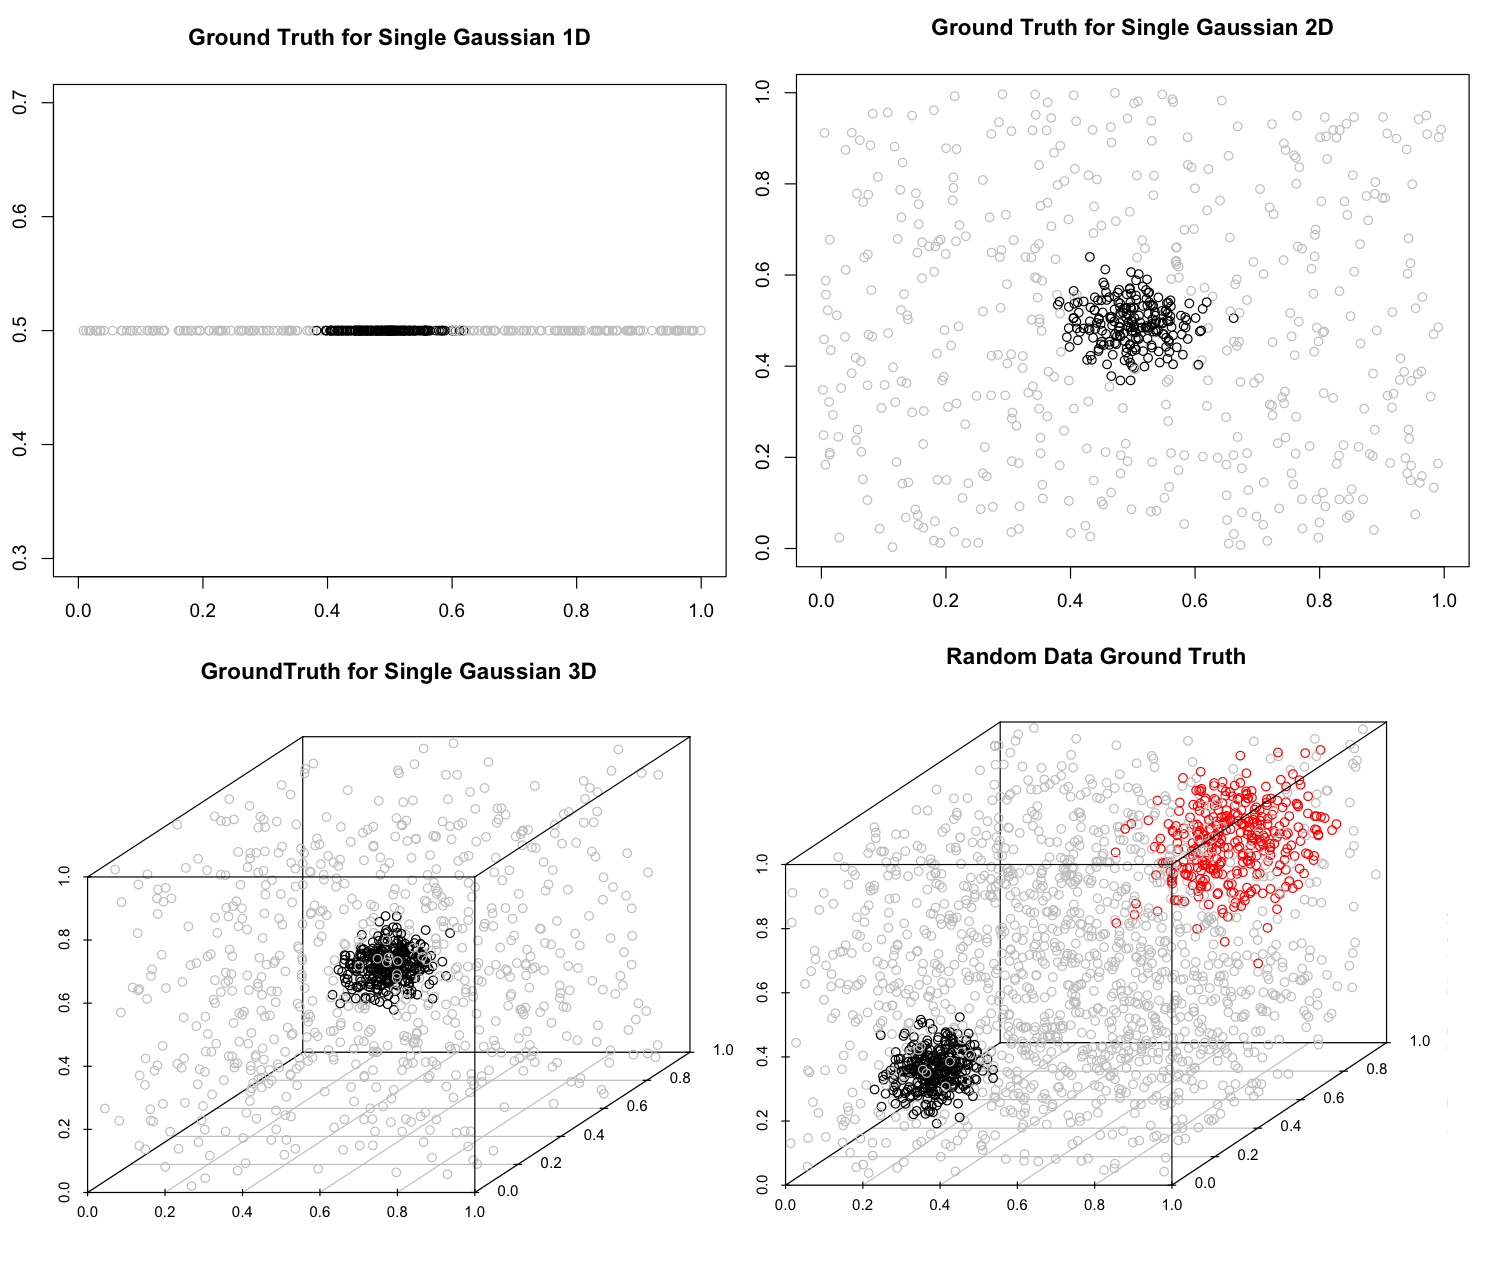
\includegraphics[width=\textwidth]{images/fourGTs}
\caption{Ground Truth values for 4 different synthetic data tests.}
\label{fig:fourGTs}
\end{figure*}

\begin{figure*}[t]
\centering
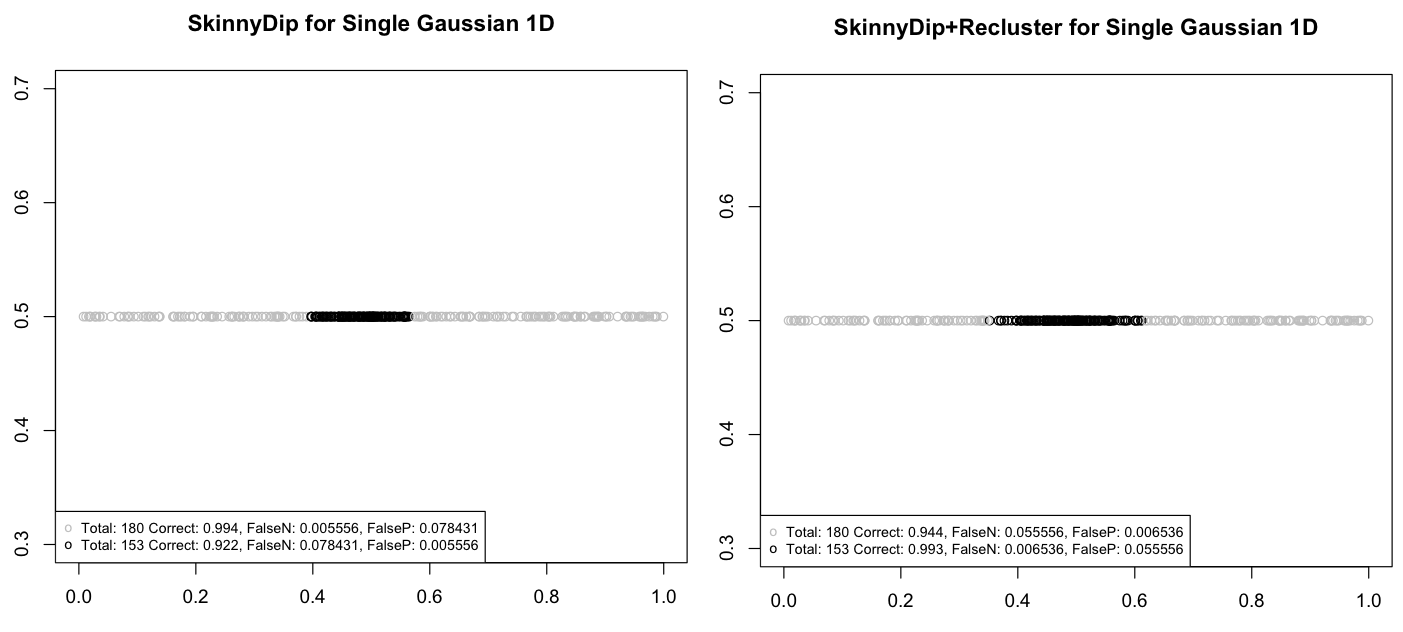
\includegraphics[width=\textwidth]{images/1Dcompare}
\caption{Comparison of SkinnyDip results before and after reclustering in 1 dimension.}
\label{fig:1Dcompare}
\end{figure*}

\begin{figure*}[t]
\centering
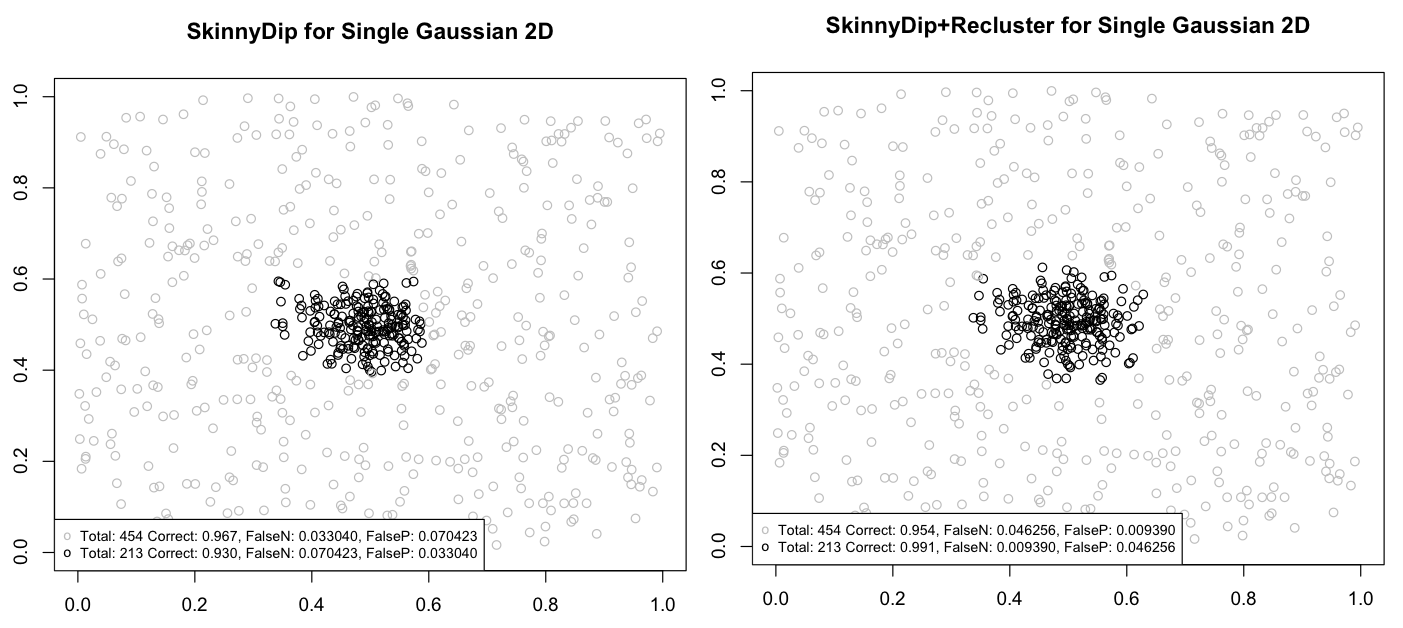
\includegraphics[width=\textwidth]{images/2Dcompare}
\caption{Comparison of SkinnyDip results before and after reclustering in 2 dimensions.}
\label{fig:2Dcompare}
\end{figure*}

\begin{figure*}[t]
\centering
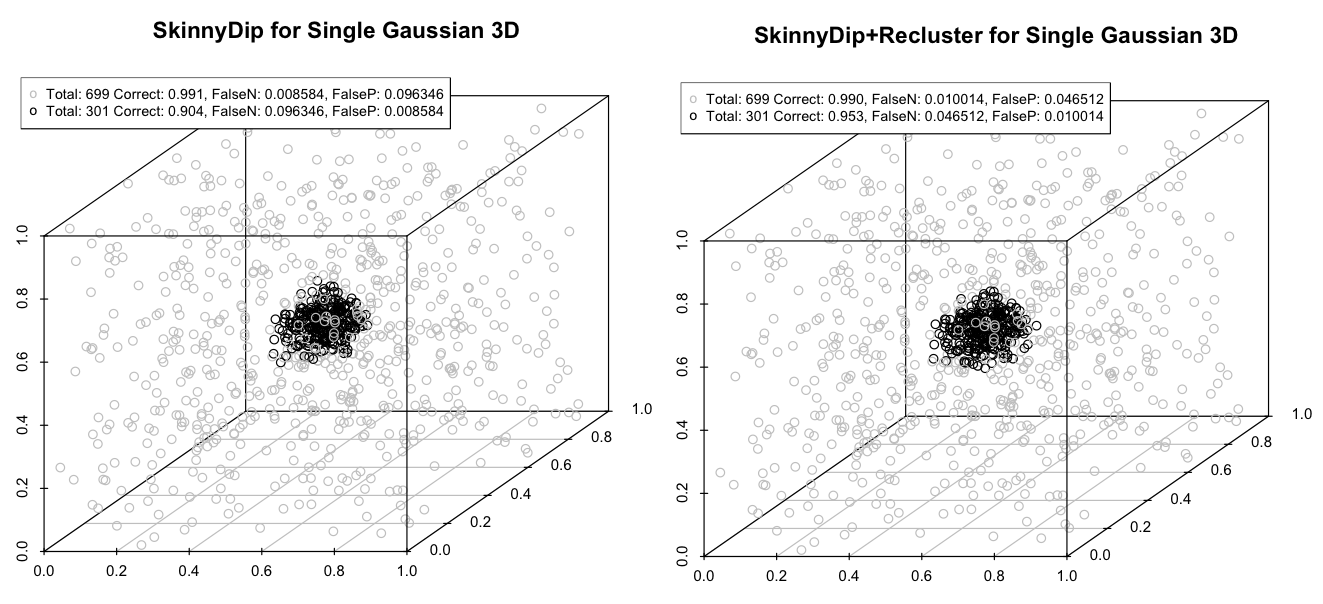
\includegraphics[width=\textwidth]{images/3Dcompare}
\caption{Comparison of SkinnyDip results before and after reclustering in 3 dimensions.}
\label{fig:3Dcompare}
\end{figure*}

\begin{figure*}[t]
\centering
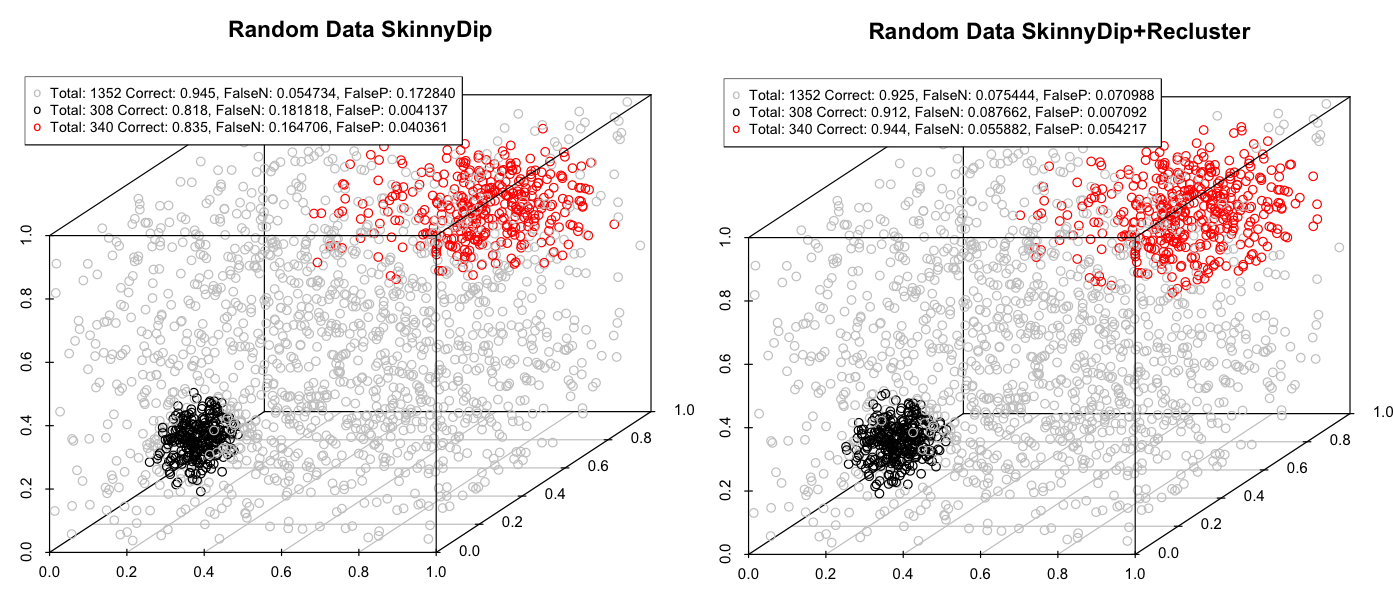
\includegraphics[width=\textwidth]{images/multicompare}
\caption{Comparison of SkinnyDip results before and after reclustering multiple 3D clusters.}
\label{fig:multicompare}
\end{figure*}

\begin{figure*}[t]
\centering
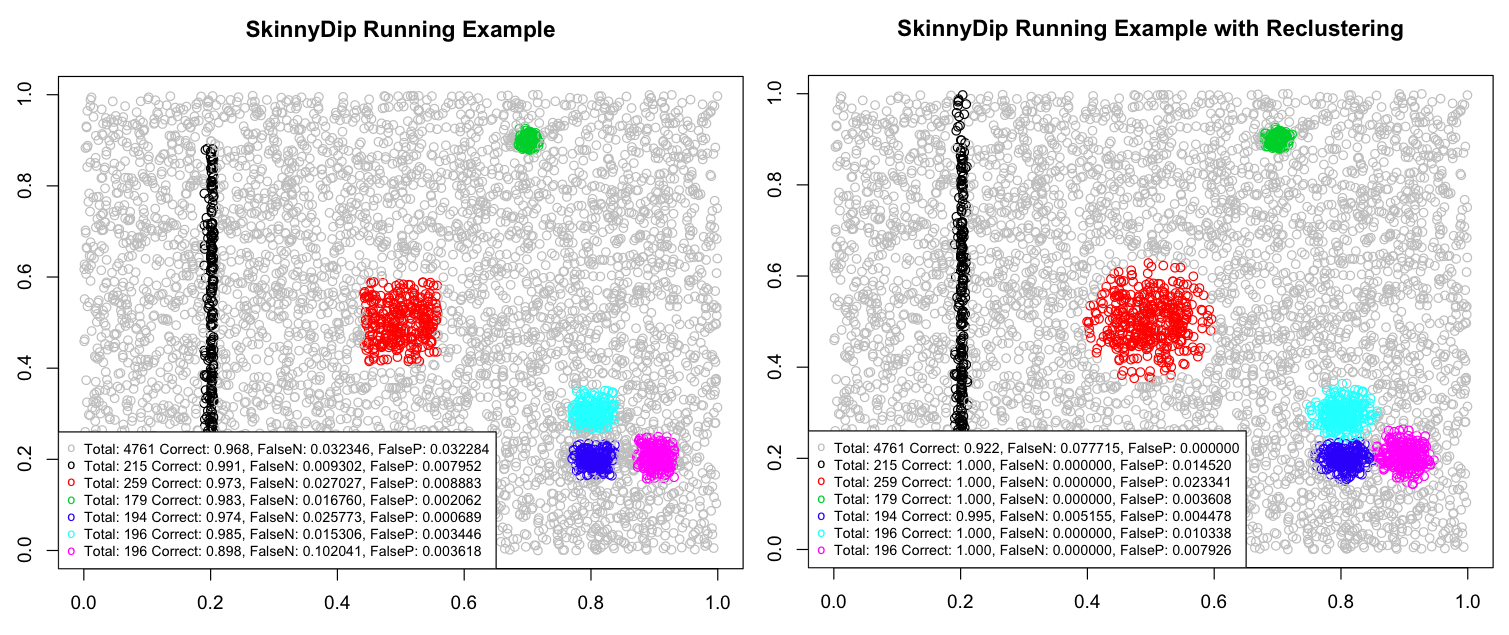
\includegraphics[width=\textwidth]{images/Runningcompare}
\caption{Comparison of SkinnyDip results before and after reclustering in the running example.}
\label{fig:runningcompare}
\end{figure*}

\begin{figure*}[t]
\centering
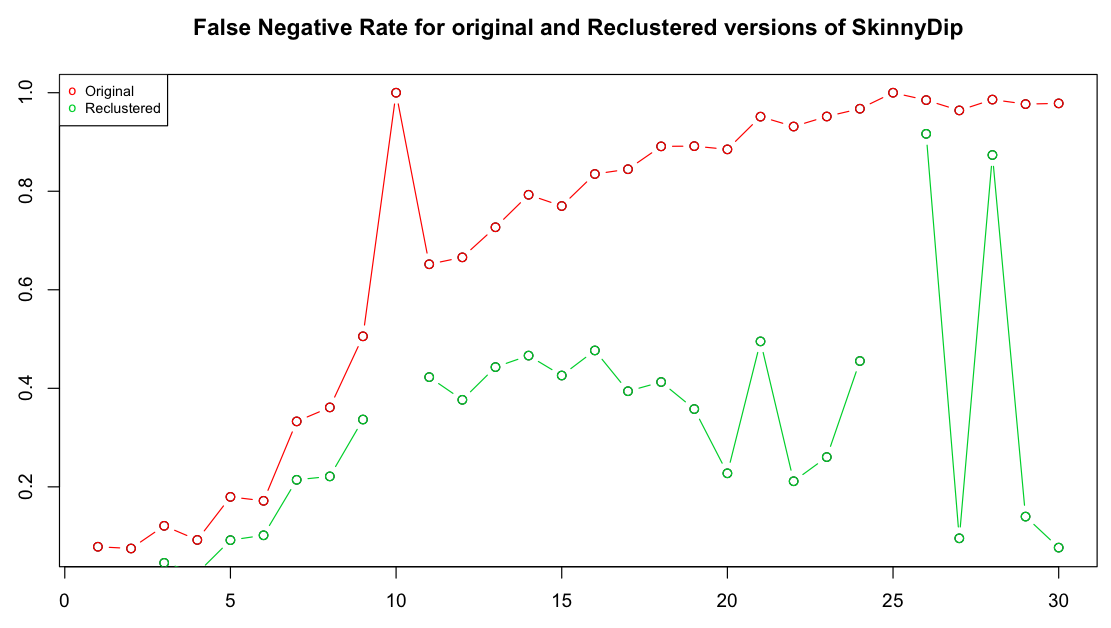
\includegraphics[width=\textwidth]{images/falsenegmd}
\caption{False Negative Rates for synthetic data in 1-30 dimensions.}
\label{fig:falsenegmd}
\end{figure*}

\begin{figure*}[t]
\centering
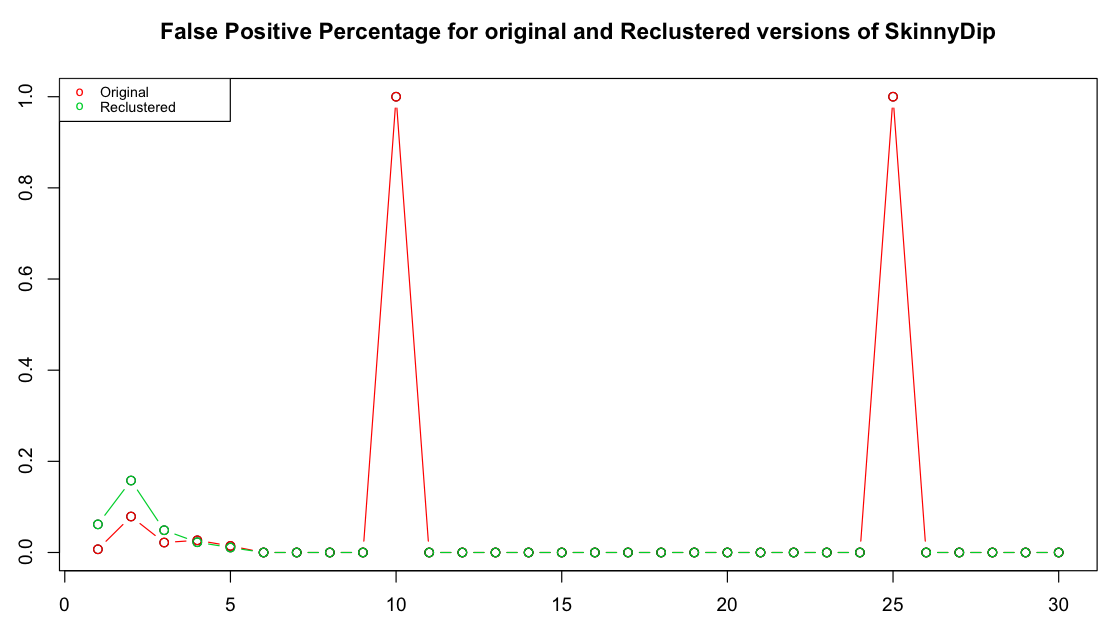
\includegraphics[width=\textwidth]{images/falseposmd}
\caption{Percentage of detected points that were noise for synthetic data in 1-30 dimensions.}
\label{fig:falseposmd}
\end{figure*}


\section{Results} \label{results}
After creating a tool to visualize the ground truth labels for these datasets, I plotted the running example from \cite{skinnydip} to see the actual underlying shape and content of the data. This is where it becomes clear that the SkinnyDip algorithm results in Figure \ref{fig:sdexample} are clipping off the ends of each dimension for clusters that are not axis-aligned squares when compared to the ground truth in Figure \ref{fig:runningGT}. After this confirmation of the type of error, I turn to the results from testing reclustering on my own synthetic data. For reference, the ground truth plots of each of these four tests are shown in Figure \ref{fig:fourGTs}.

The first of these tests is a unimodal distribution with random noise from a uniform distribution in the background. Figure \ref{fig:1Dcompare} shows that we have 7.84\% of points being misclassified as background noise before reclustering, and this is reduced to 0.543\% after reclustering. The second image is much more visually similar to the ground truth example, giving a small amount of evidence that it represents a more accurate picture of the underlying data. In this test case, the False Positive rate for the cluster increases by a factor of 10 during this reclassification, from 0.556\% to 5.556\%. This is a significant jump, but the effect decreases as we increase our data's dimensionality. It is important to note that we still have both false negative and false positive values in the 1D case due to the structure of the data described in Section \ref{data}. This buffer zone means that, for this data, it will almost always be impossible to have a perfectly classified cluster.

In the second dimension, we have a cluster defined by a multivariate Gaussian centered in the middle of a field of noise. When testing and reclustering this example (see Figure \ref{fig:2Dcompare}), we see our cluster's false negative rate drop from 7.04\% to 0.939\%. In this case, the False positive rate for the cluster remains fairly stable, changing from 3.30\% to 4.63\% after reclustering. In the associated images, we can see portions of the cluster being 'rounded off' through reclustering now, particularly along the top and left edges of the cluster.

For the first three dimensional example, we still have a single multivariate Gaussian cluster, but it becomes a bit harder to visualize. On the 3D scatterplot (Figure \ref{fig:3Dcompare}) we do not really see much of a change in the visual structure of the cluster, though there might be visible changes when viewed from another angle. However, the reported stats still allow us to know that the false negative rate dropped from 9.63\% to 4.65\% while the false positive rate only rose from 0.858\% to 1.00\%. Finally we look at a second three dimensional case to see if this effect is reproducible in multiple clusters simultaneously.

Our fourth test includes two multivariate Gaussian clusters of different sizes and distributions, as can be seen in Figure \ref{fig:multicompare}. In this case, we can see the shape of the larger, red cluster change a bit, appearing to form a more elliptical shape. The false negative rate for the smaller, black cluster drops from 18.2\% dropping to 8.77\% while the false positive rate rises from 0.414\% to 0.709\%. The larger cluster also experiences a substantial drop in false rejection, with a false negative rate of 16.5\% to 5.59\% after reclustering, while the false positive rate rose from 4.04\% to 5.42\%. We can also see the false positive classification rate for the background noise dropping by over 10\% because of this improvement.

Given that it is impossible to visualize clusters at higher dimensions, the remaining tests in higher dimensional spaces are reported entirely based on error rates. I ran a series of increasingly multidimensional test data through both SkinnyDip and reclustering steps and calculate error rates for each. The first metric reported is the false negative rate for clusters in each dimension (See Figure \ref{fig:falsenegmd}. The second metric being reported is no longer the false positive rate across the entire dataset, but the percentage of detected points that were false positives, also known as the false discovery rate. This plot (Figure \ref{fig:falseposmd}) allows us to have a better visual of the percentage of points erroneously included in a cluster as the dimension increases.

There are two outliers in these plots, at a dimensions 10 and 25. These are cases where the SkinnyDip algorithm failed to report a cluster, and therefore we have complete classification failure. Reclustering data was not shown for these two cases in either plot. We can see that reclustering consistently reduces error as dimension increases, with an increasing effect as we pass beyond 10 dimensions. The data begins to get quite erratic, however, after about 20 dimensions. In Figure \ref{fig:falseposmd}, we see that the reclustered data has more false discoveries, which is consistent with the 1, 2, and 3 dimensional data reported above. Interestingly, it appears that this error rate decreases in higher dimensions, and is essentially zero for for dimensions beyond 5. This would indicate to me that the the new clusters in higher dimensions are fully contained within the ground truth distribution. This may indicate that the base that I use to exponentially grow my Mahalanobis threshold is too small, as the reclustered areas are growing at a rate slower than the underlying distributions.

Because we are exponentially increasing the amount of data that we are approximating with the Mahalanobis distance method, the estimation loses stability, and has the risk of bulging or shrinking the multivariate Gaussian in dimensions that are not appropriately represented in the increasingly small subset of the cluster being sampled. This may contribute to the instability of the error reduction shown in \ref{fig:falsenegmd}, as at this point, the SkinnyDip cluster used as evidence represents less than 10\% of the true cluster points.

Returning to the running example data set, we can now test to see how the reclustering algorithm changes the detected regions. In Figure \ref{fig:runningcompare}, we can see that reclustering actually reduces the false negative rate for all clusters to 0\%, except for the blue cluster, the middle cluster of the three in the bottom right region of the image. However, this cluster likely only has its 0.516\% false negative rate due to the fact that the cyan cluster above it has dominated it and taken over all points in their intersection were classified to the cyan cluster. This has to do with the cluster by cluster order in which points are classified and is a noted flaw in this method. 

That being said, if we look at the ground truth for this data in \ref{fig:runningGT}, it appears that these clusters actually do have an overlap. This comes from the fact that the authors used a different method to generate their synthetic labels. Only points within the ~95\% Confidence Interval were added to a cluster, and points generated by the underlying distribution outside of this range were labeled as noise instead. This also explains why the false negative rates are dropping to 0\%, compared to my tests. Had my tests discarded the tails of their distributions as noise or had the running example data set included them in the cluster, I believe the results would have been even more similar. This shows that my algorithm is overclassifying into into its target distribution in 2D data.

The other result that we see in the running example data is how poorly my algorithm performs on hypercubic regions. Because it makes the assumption that the underlying data is normally distributed, these hypercubic regions are turned spherical, in the case of the red cluster, or elongated in the case of the black cluster. In these cases evidence captured in these hypercubic regions is actually representative of the cluster, but the covariance matrix will approximate it as extended past these bounds relative to how variant the data is in that direction. This indicates that this method is ill-suited for distributions that are not Gaussian in nature.

\section{Conclusion}
As expressed by the authors in the paper, SkinnyDip is a very fast, accurate, deterministic way of finding clusters in uniform noise. My tests on the authors' data and my own synthetic data ran very quickly and always came up with identical results on separate runs. The original SkinnyDip algorithm, however, is prone to falsely rejecting points from clusters that are not hypercubic, a uniform shape that not likely to occur in real-world data. It is also not well-suited to noisey data in high dimensions, which we observed through the False Negative Rate approaching 100\% as dimensionality increased. Both of these issues were improved by using the existing cluster memberships as evidence for the covariance of the underlying distribution and reclustering with Mahalanobis distance under a threshold that increases exponentially with dimension of the data.

My clustering addition was applied to SkinnyDip, and tested on fairly ideal data in normal space. However, the same SkinnyDip clustering is used in SparseDip, after data has been projected into a maximally modal space, and in theory, the same reclustering method is an equally viable addition there.

\subsection{Risks}

My algorithm is offline, so points that are initially present in one cluster are accounted for when calculating its covariance, even if they are later reassigned to be in another cluster. This type of conflict will occur when clusters are sufficiently close together or have a sufficiently wide distributions (consider a bimodal distribution that does not reach reach its minimum value between peaks). In this case, the cluster with a higher label in ground truth ordering will take precedence, and all points in the intersection will be assigned to this cluster. Note that this conflict will not occur with the SkinnyDip clusters themselves, they will either be merged, or separate enough that there is no overlap; the conflict only occurs when we try to extend the membership of the cluster.


\section{Future Work}
Further analysis of the covariance before reclustering could show relatively uniform noise, indicating that a hypercubic cluster region may actually be a uniform hypercube, as seen in the running example data.

The 1-30 dimension false negative rate and false discovery rate plots should be run multiple times with both different seeds and different data distributions to see how consistent and reproducible the error reduction actually is.

The real-world data tested in \cite{skinnydip} did not contain any noise at all, and k-means was used to fill out the noise left behind by Skinny/SparseDip. I did have the time to noisy real-world data to test my algorithm on. This was one of my main initial goals, and I would still like to find a dataset involving noisy positional data; I am particularly interested in galaxy clustering within star fields to test the accuracy of my augmentation to a real-world problem.

A useful altercation that could be made to my existing problem would be to partition the dataset, so that more efficient label reclassifications can be performed. It is clearly unnecessary to calculate distance measurements for all points in the dataset if the majority is noise. Finding distance measurements on a local subset of points around a cluster would increase space and time complexity of the reclassification step. This reduction in space complexity is especially important, as my calculations in R were starting to exceed maximum table capacities as the data set grew in excess of 100k points, and began using asymptotic approximations, though this was occurring within the SkinnyDip code as well.




\bibliography{final-report}
\bibliographystyle{unsrt}
\end{document}
